\documentclass[12pt]{article}
\usepackage[utf8]{inputenc}
\usepackage{listings}
\usepackage{setspace}
\usepackage{graphicx}
\usepackage{hyperref}
\usepackage{amsmath}
\usepackage{booktabs}
\usepackage{csquotes}
\usepackage{cases}
\usepackage{titling}
\usepackage{blindtext}
\usepackage{float}
\usepackage{amssymb}
\usepackage{mathtools}
\usepackage{subcaption}
\usepackage{lipsum}
\usepackage[left=2.5cm,top=2.5cm,right=2.5cm,bottom=2.5cm]{geometry}
\setlength{\parindent}{0pt}

\doublespacing
\hypersetup{
    colorlinks=true,
    linkcolor=blue,
    filecolor=magenta,      
    urlcolor=cyan,
}

%\renewcommand{\familydefault}{\sfdefault}

\title{CTA200 Assignment 3}
\author{Feiyu Quan}
\date{May 2022}


\begin{document}

\maketitle

\section{Question 1}

\begin{figure}[H]
    \centering
    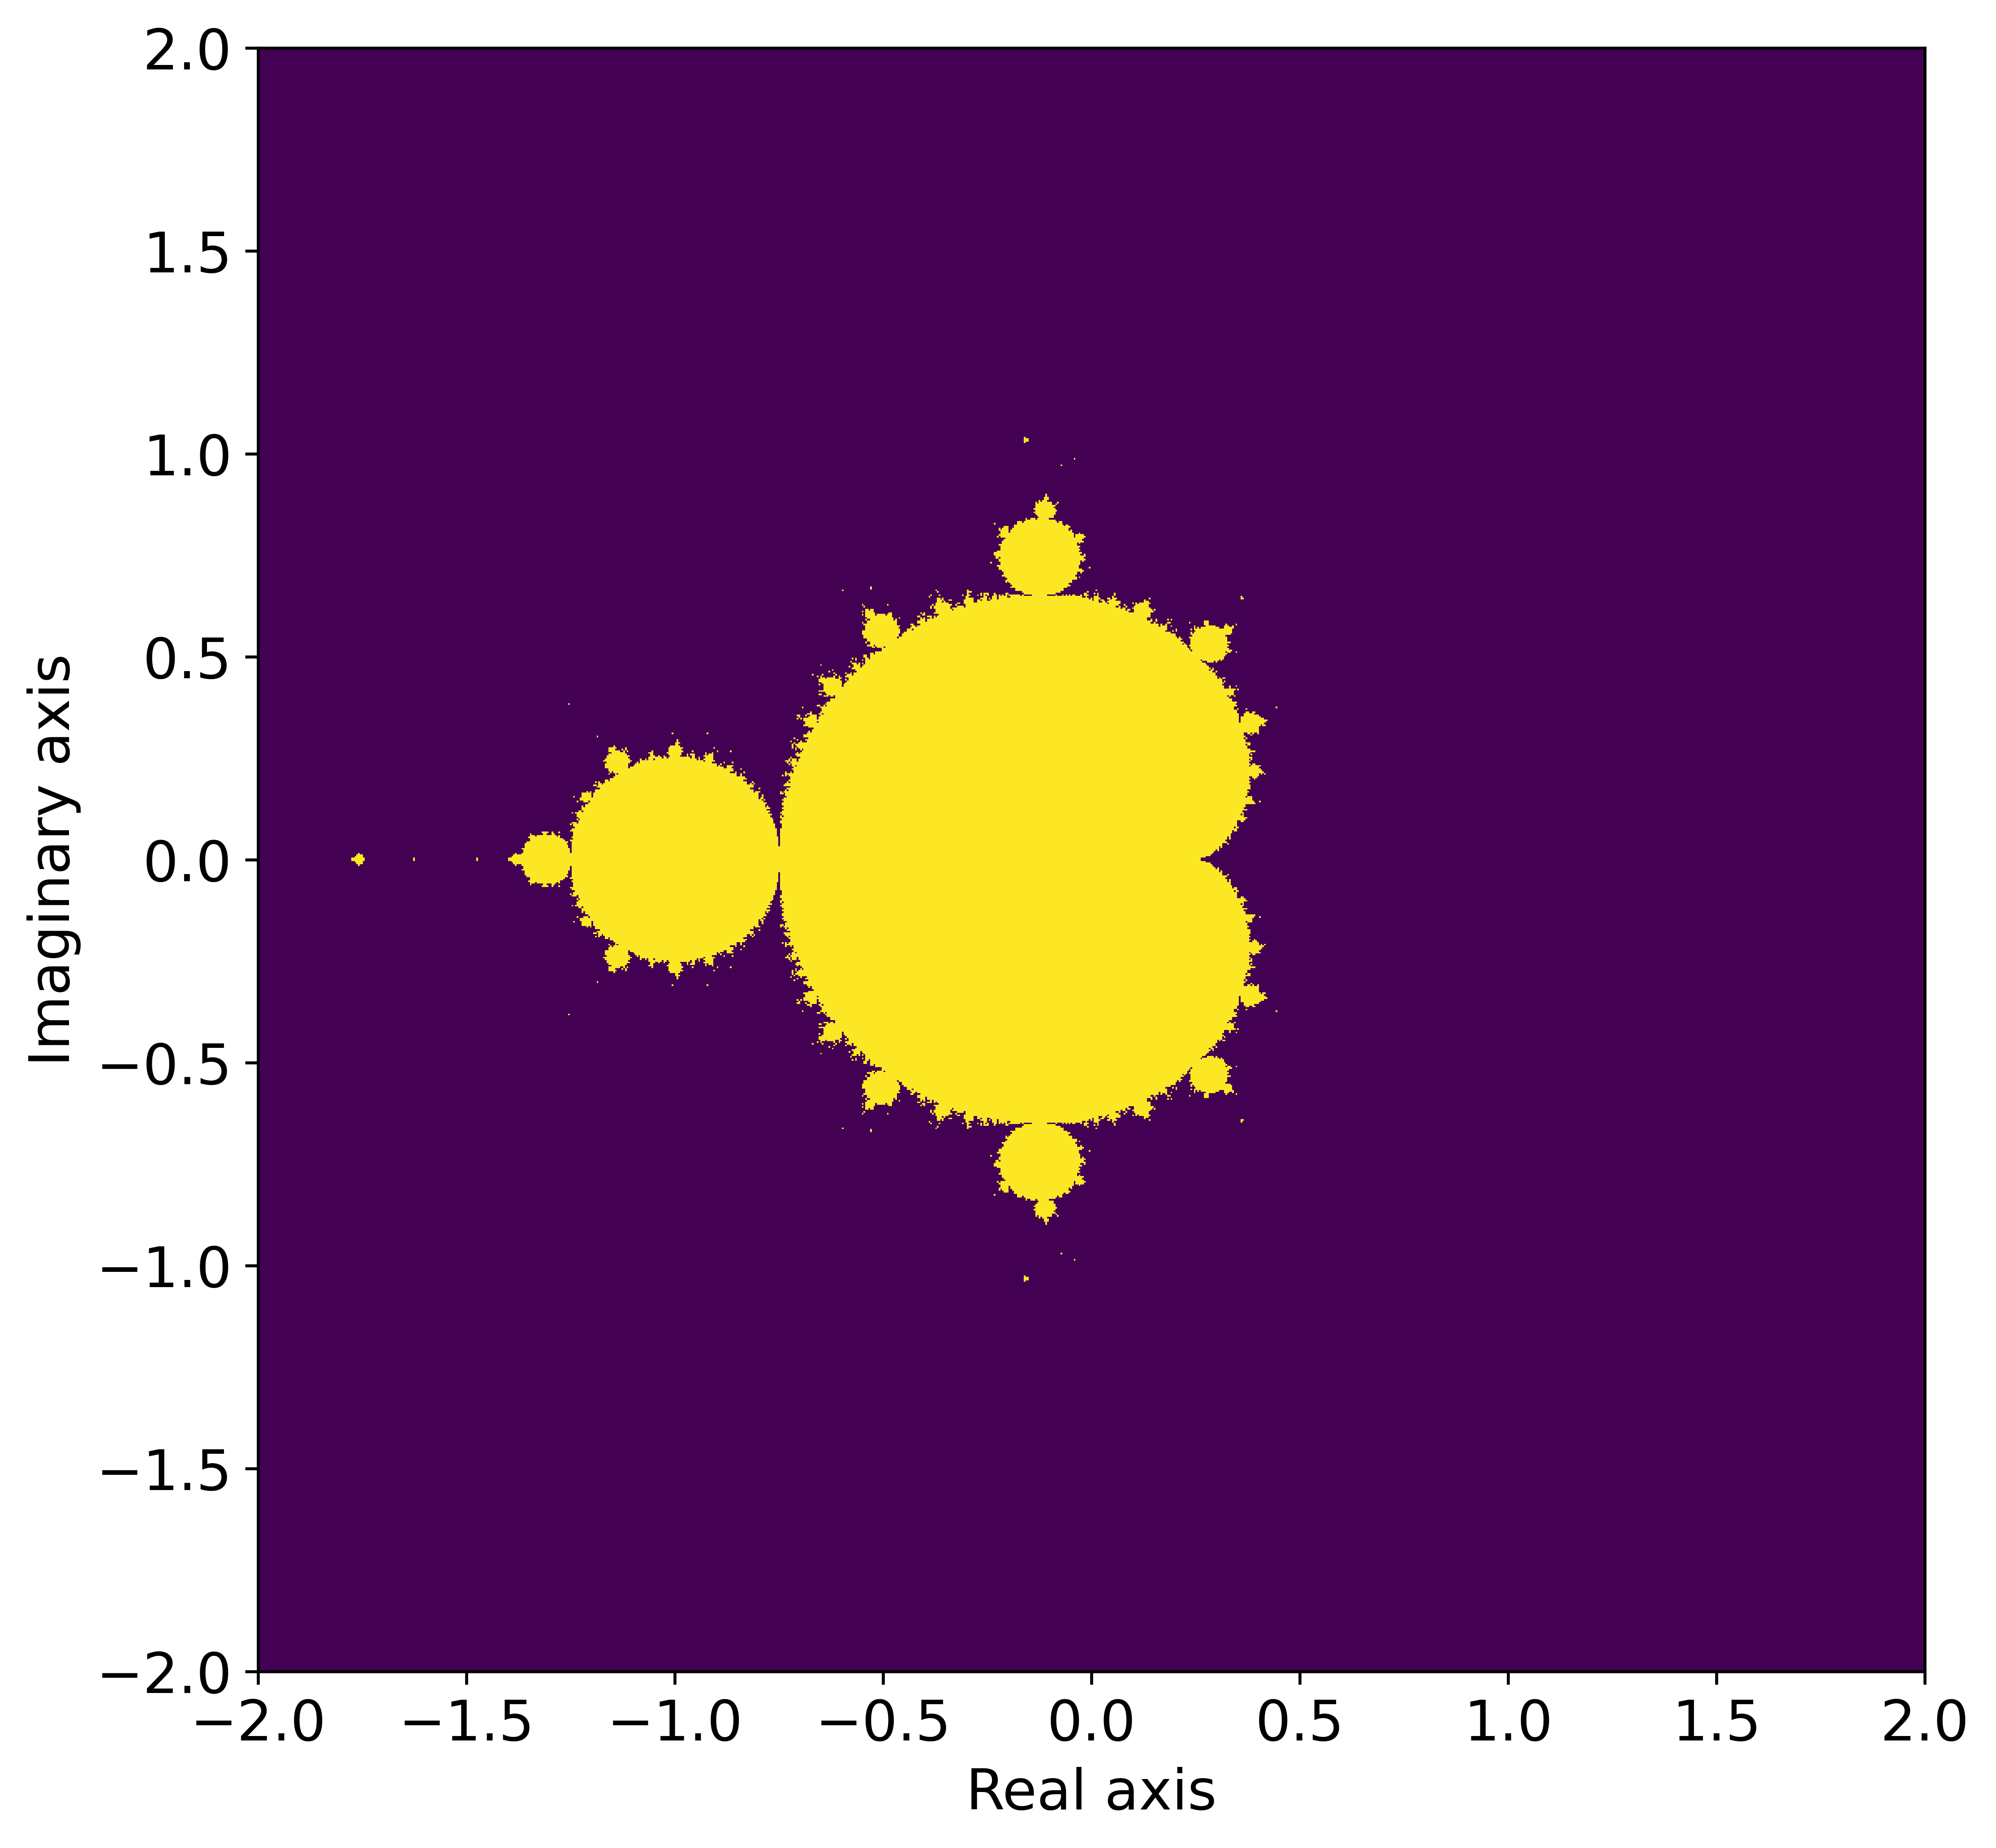
\includegraphics[scale = 0.7]{Figure_1.png}
    \caption{Plot of the Mandelbrot set. Converging points are labelled yellow while diverging points are labelled purple.}
\end{figure}

\begin{figure}[H]
    \centering
    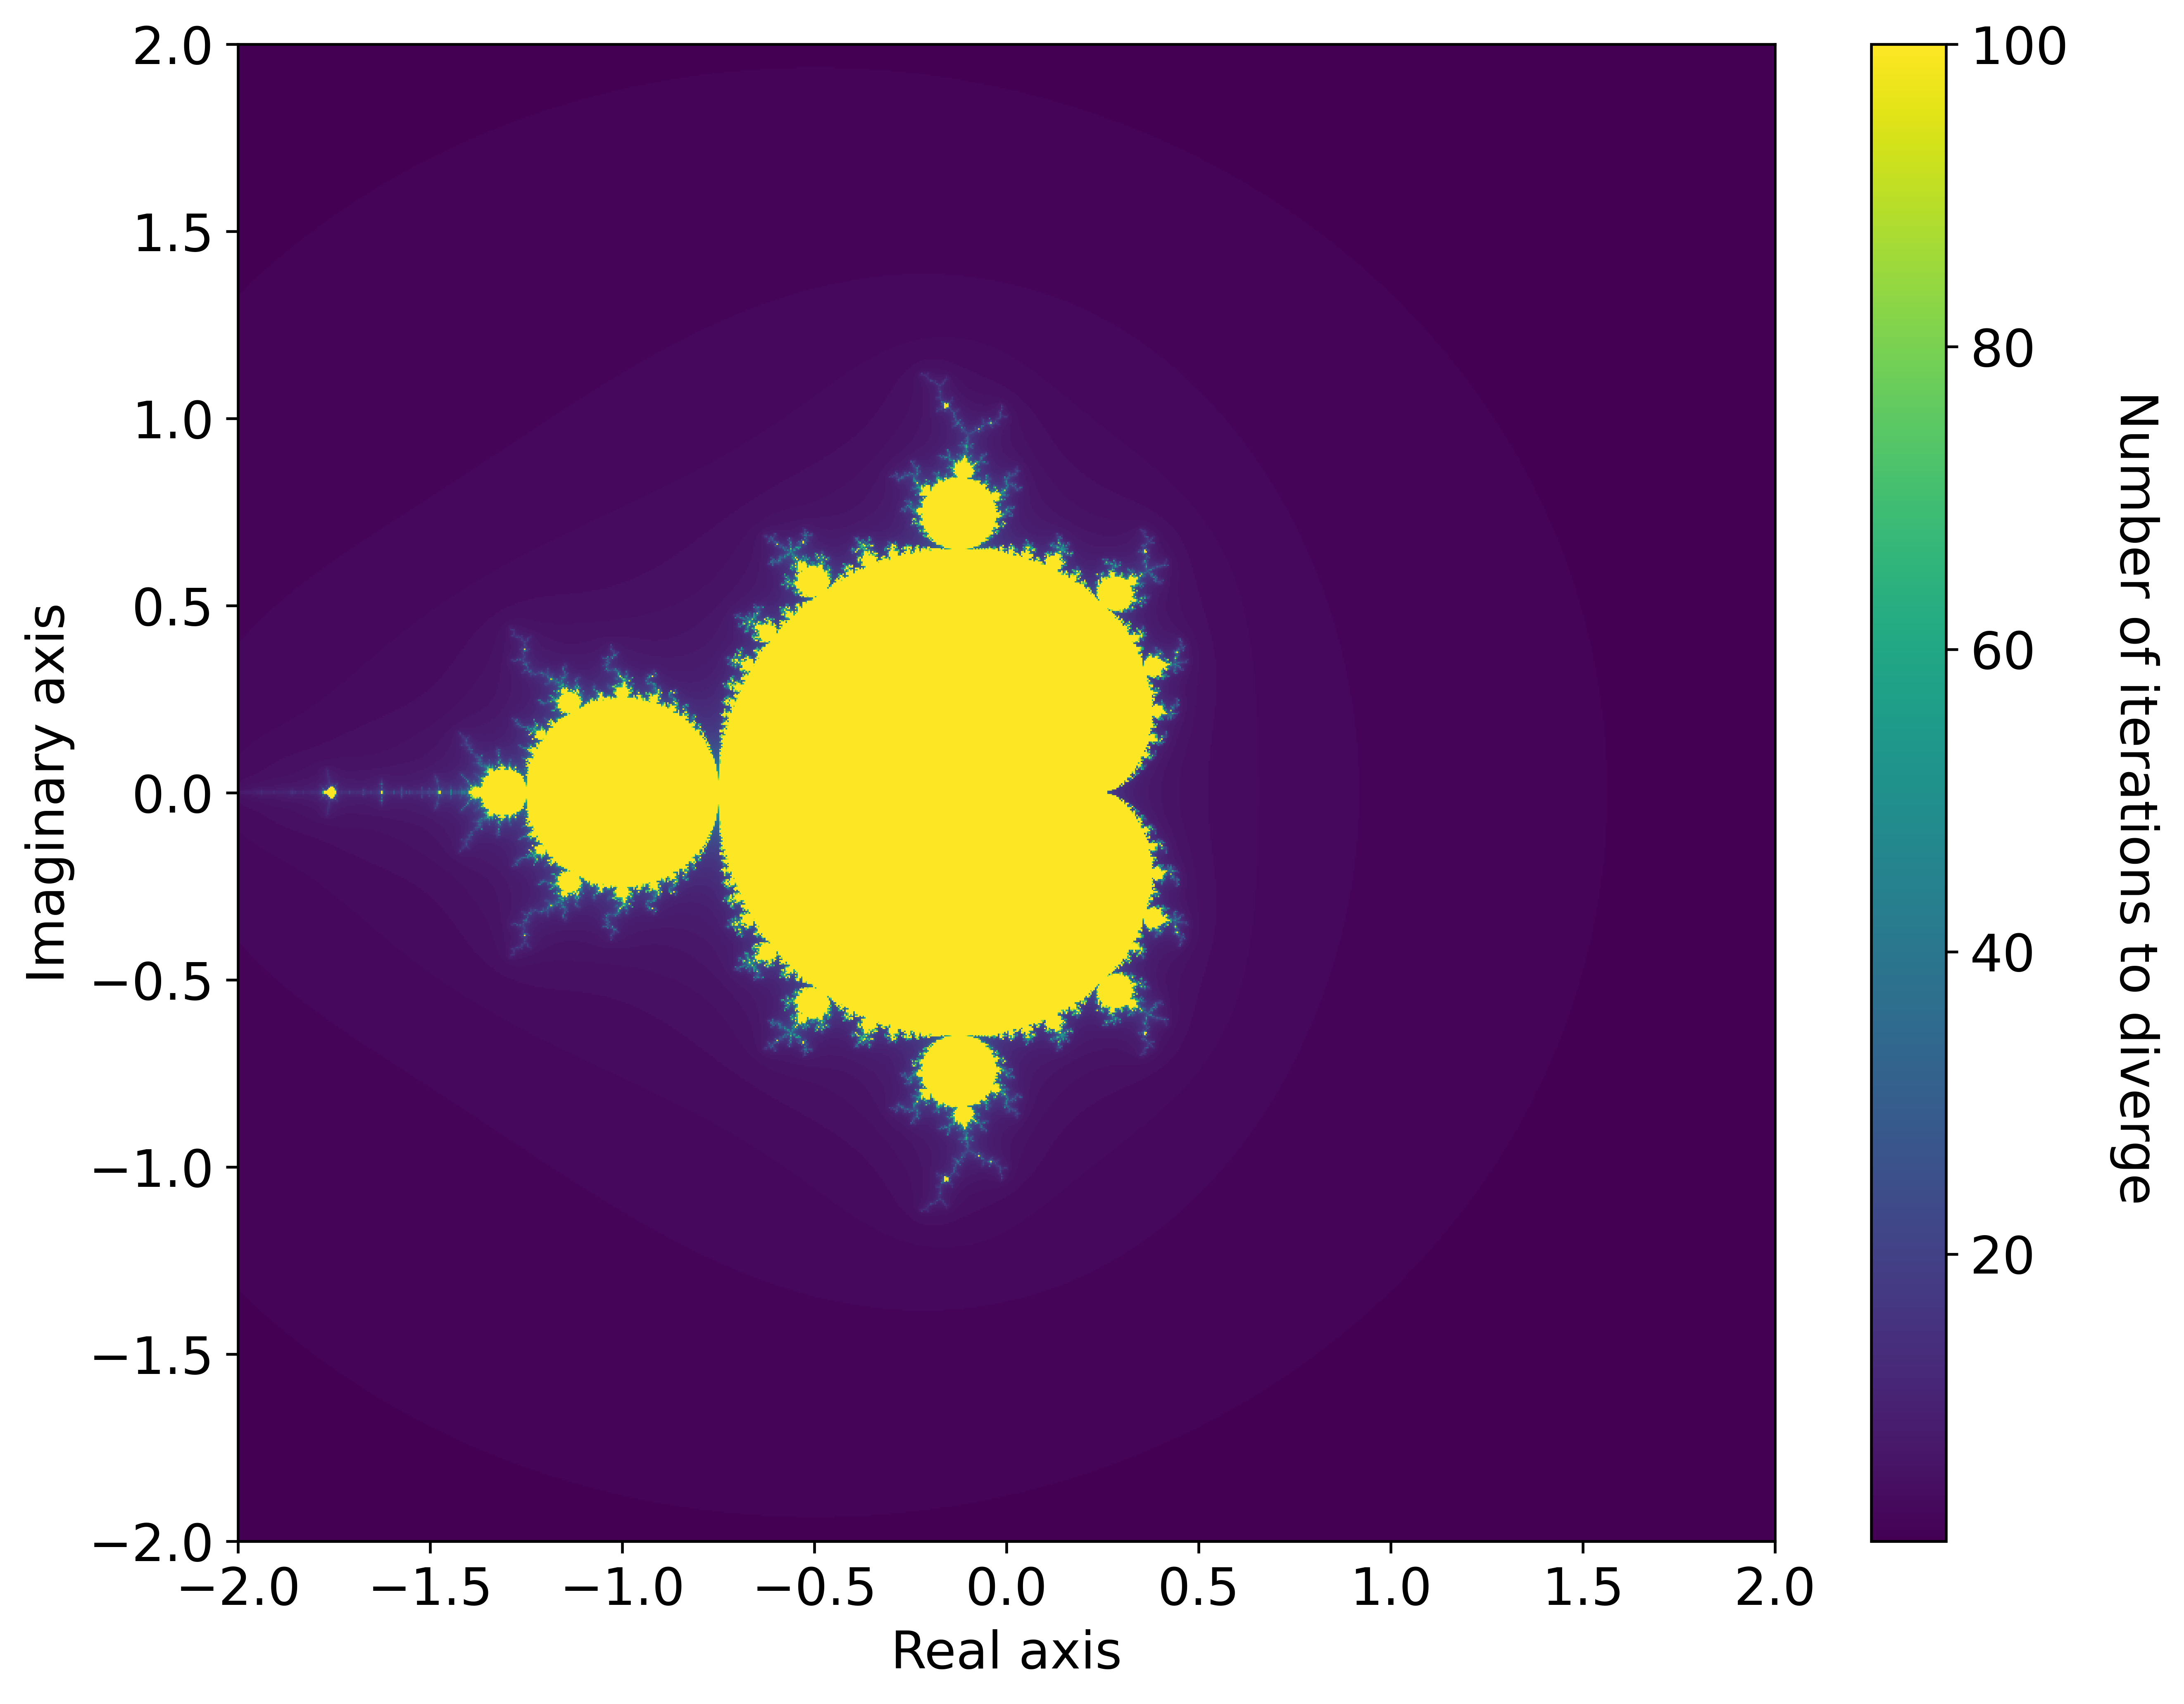
\includegraphics[scale = 0.7]{Figure_2.png}
    \caption{Similar to Figure 1, but the diverging points are labelled based on a color scale by the number of iterations it takes for the point to diverge, as shown on the right.}
\end{figure}

The question asks us to plot the Mandelbrot set, based on classification of divergence of points when applied to the formula $z_{n+i} = z^2_n + c$, with starting point $z_0 = 1$. For each complex number $c = x + yi$ in the domain $-2 < x < 2$ and $-2 < y < 2$, we iterate them for at most 100 times to see if they diverge from the above domain, by checking if $|z| > 4$. Figure 1 shows the result of plotting those diverging points as purple points, and converging points as yellow points. Figure 2 shows the rate of divergence for all the points, by labelling points according to a color scale. Closer to the purple end, the points are diverging faster; while closer to the yellow end, the points are diverging slower. The points in the central yellow region are converging.


\section{Question 2}

Our task is to solve the following coupled differential equations:

$$
\begin{aligned}
\dot{X} &=-\sigma(X-Y) \\
\dot{Y} &=r X-Y-X Z \\
\dot{Z} &=-b Z+X Y
\end{aligned}
$$

Figure 3 shows the numerical solution of the Y equation as a function of time, with initial conditions $W_{0}=[0 ., 1 ., 0 .]$ and  and parameters $[\sigma, r, b]=$ $[10 ., 28,8 . / 3 .]$. Figure 4 shows the phase space of the numerical solutions.

\begin{figure}[H]
    \centering
    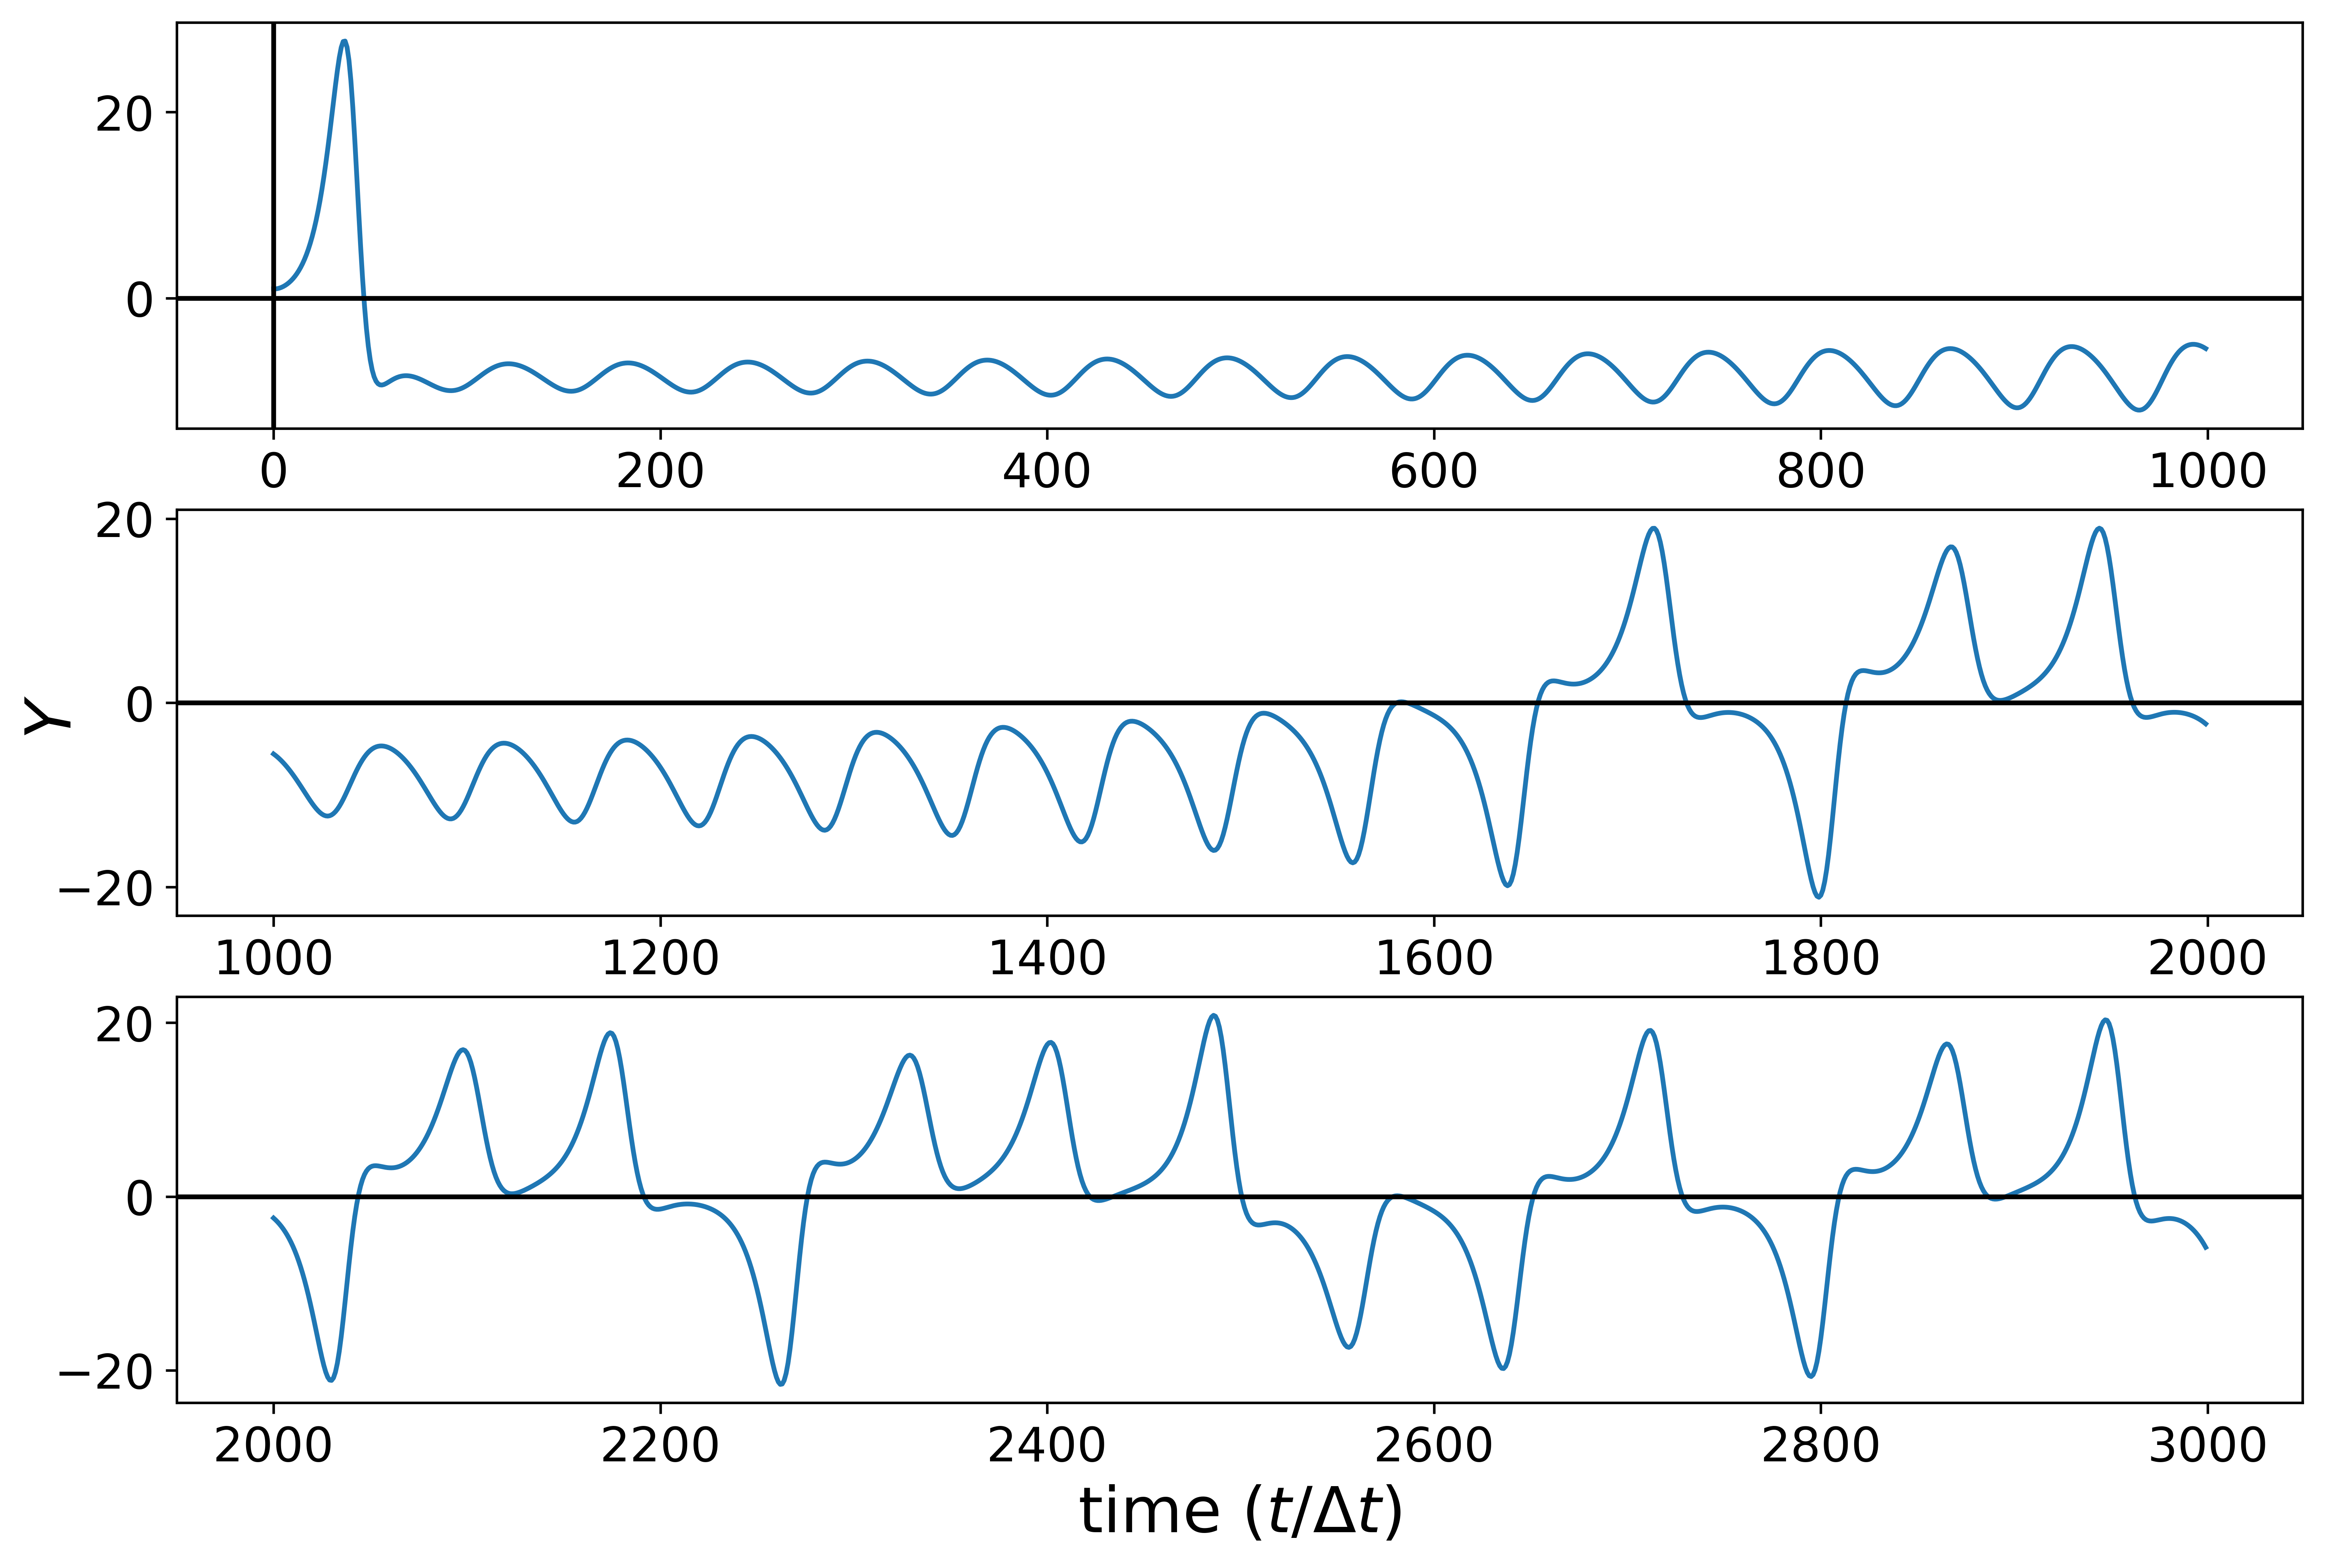
\includegraphics[scale = 0.6]{Figure_3.png}
    \caption{Reproduced Figure 1 from Lorenz (1963).}
\end{figure}


\begin{figure}[H]
    \centering
    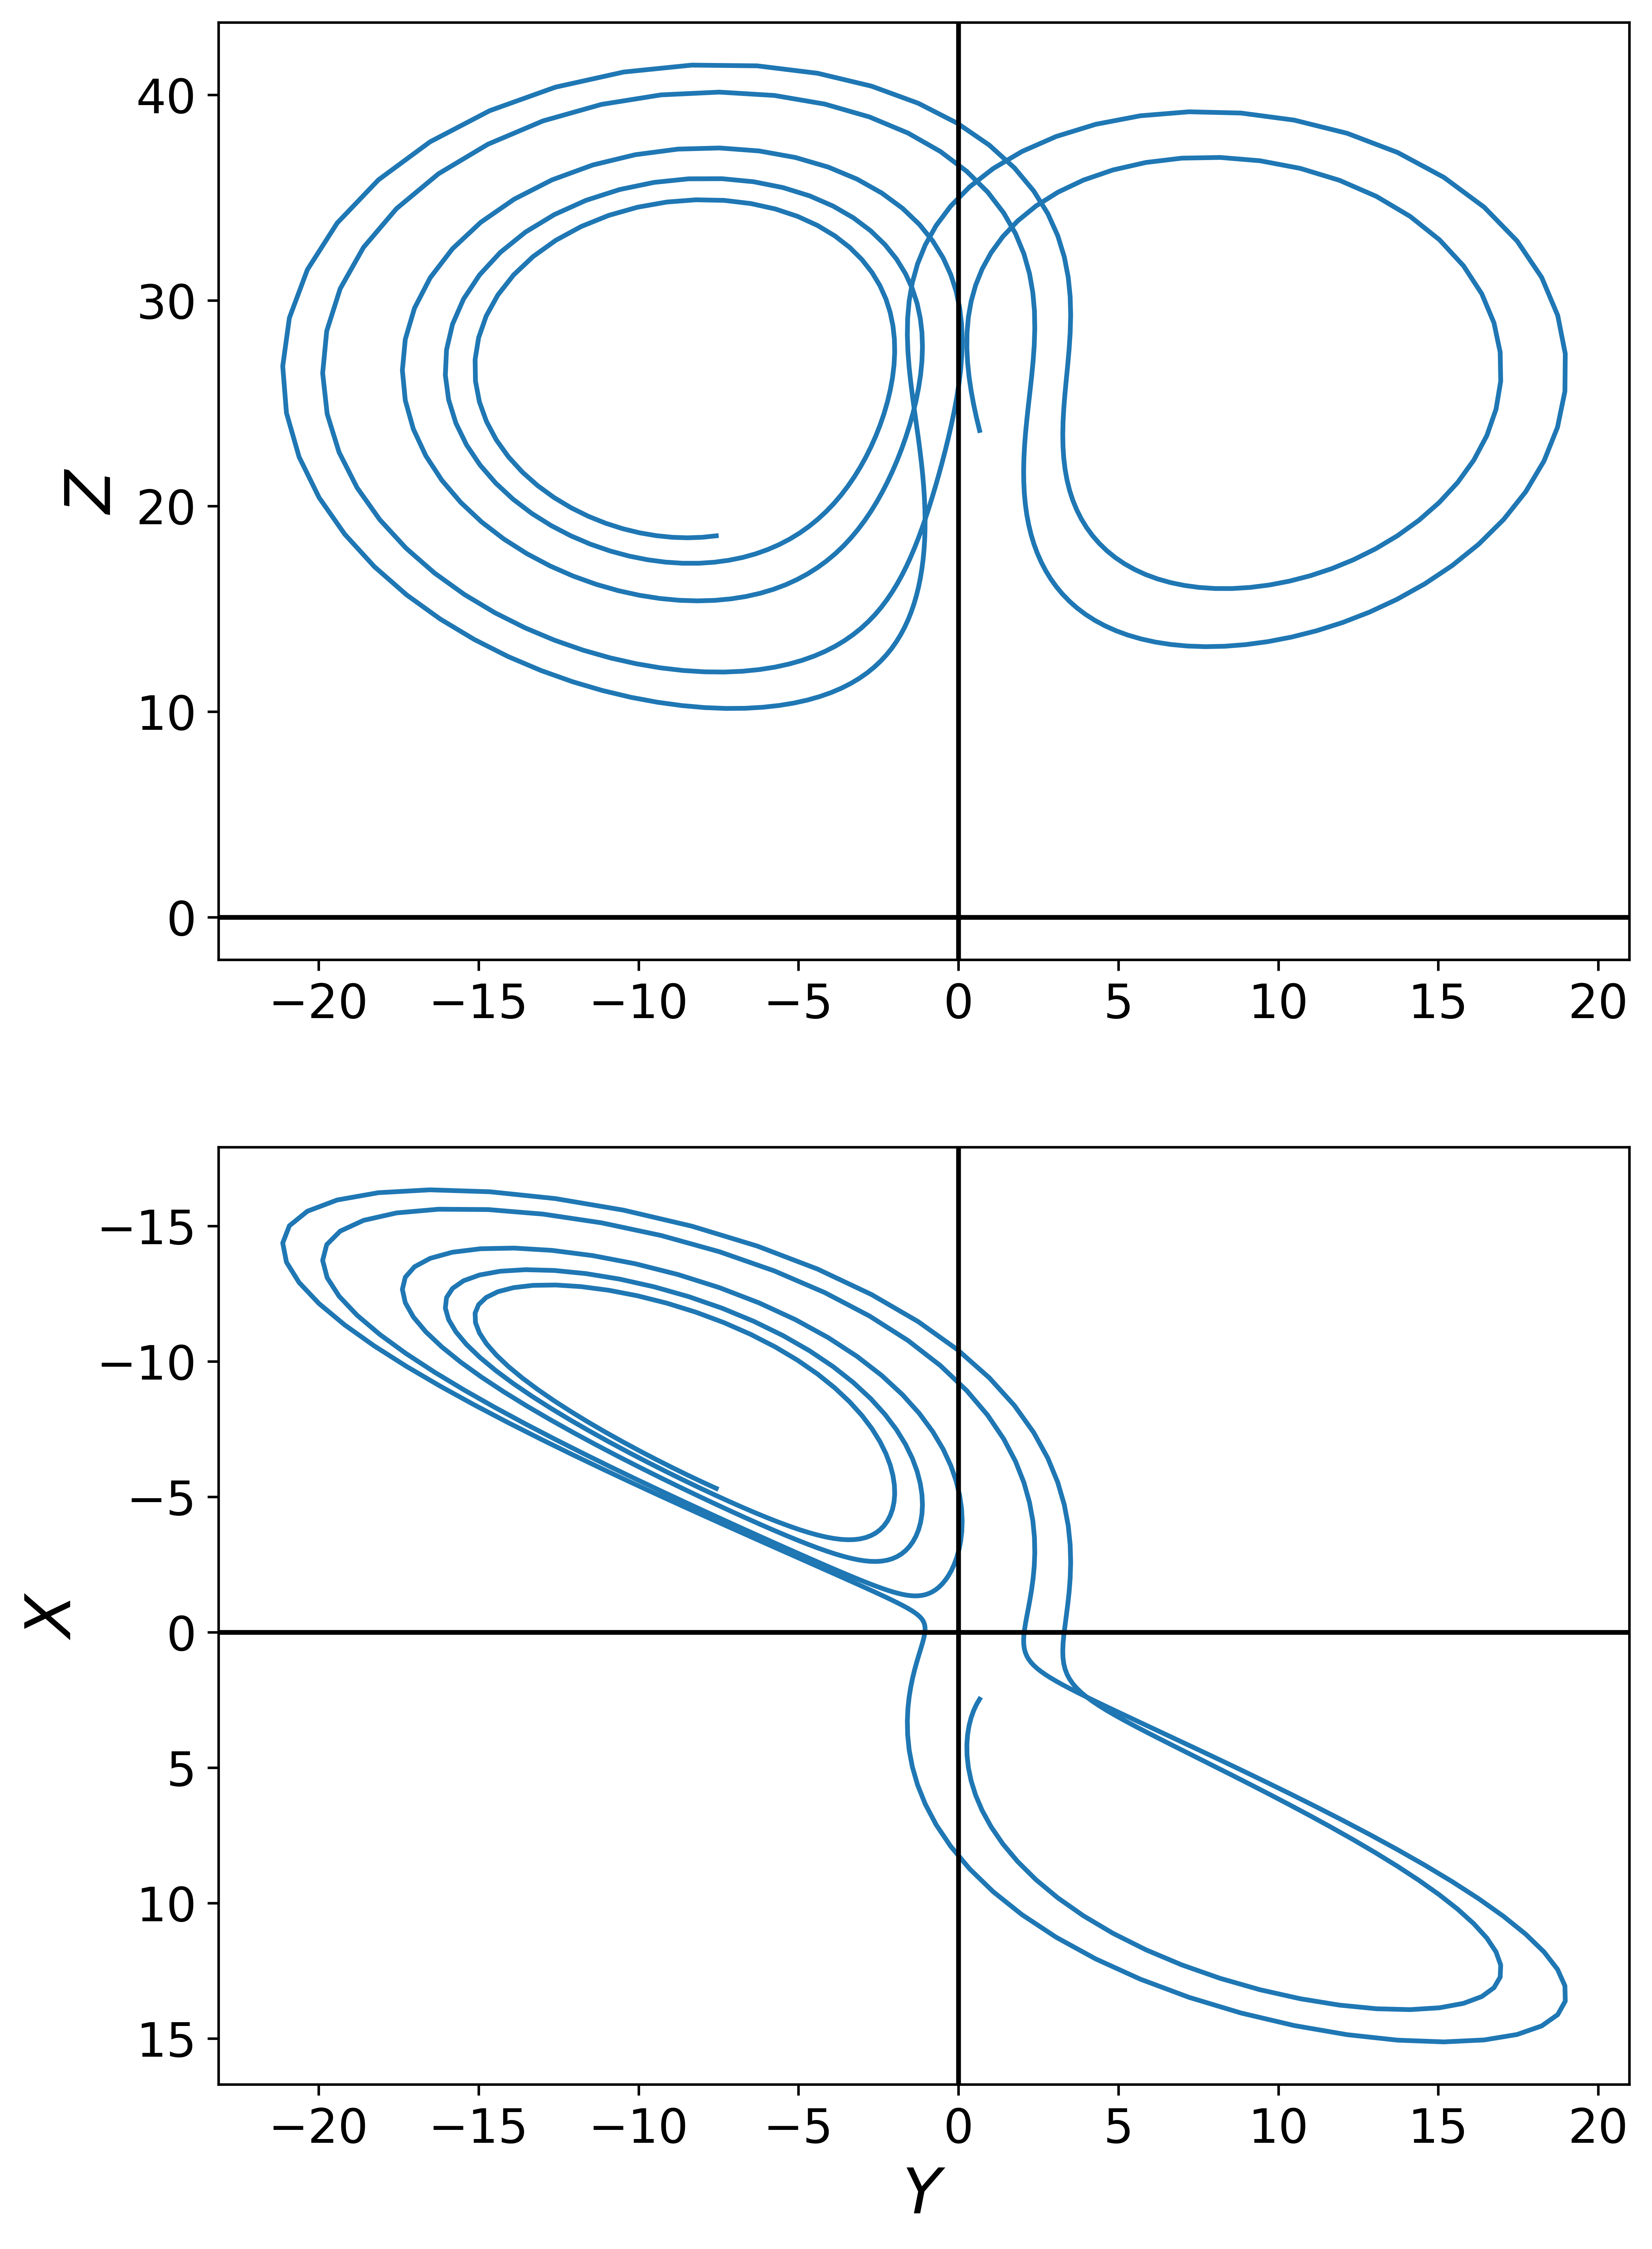
\includegraphics[scale = 0.7]{Figure_4.png}
    \caption{Plot of Lorenz attractors. Reproduced Figure 2 from Lorenz (1963).}
\end{figure}

We noticed that Figure 3 and 4 are not exactly the same as Figure 1 and 2 from from Lorenz (1963), although they are qualitatively similar. One of the possible explanations is that since we are numerically solving a chaotic system, any slight deviation in the methods we use could lead to different final results. This deviation could be that the numerical precision at Lorenz's time is not as good as that on a modern computer today, or that Lorenz used a different integrator compared with the \texttt{SciPy odeint} integrator we use.

We now change the initial conditions to $W_{0}=[0 ., 1. + 1e-8, 0 .]$, which is a small difference from the previous conditions $W_{0}=[0 ., 1., 0 .]$. We then solve the system based on this new set of conditions, and plot the difference of the two numerical solutions in Figure 5.

\begin{figure}[H]
    \centering
    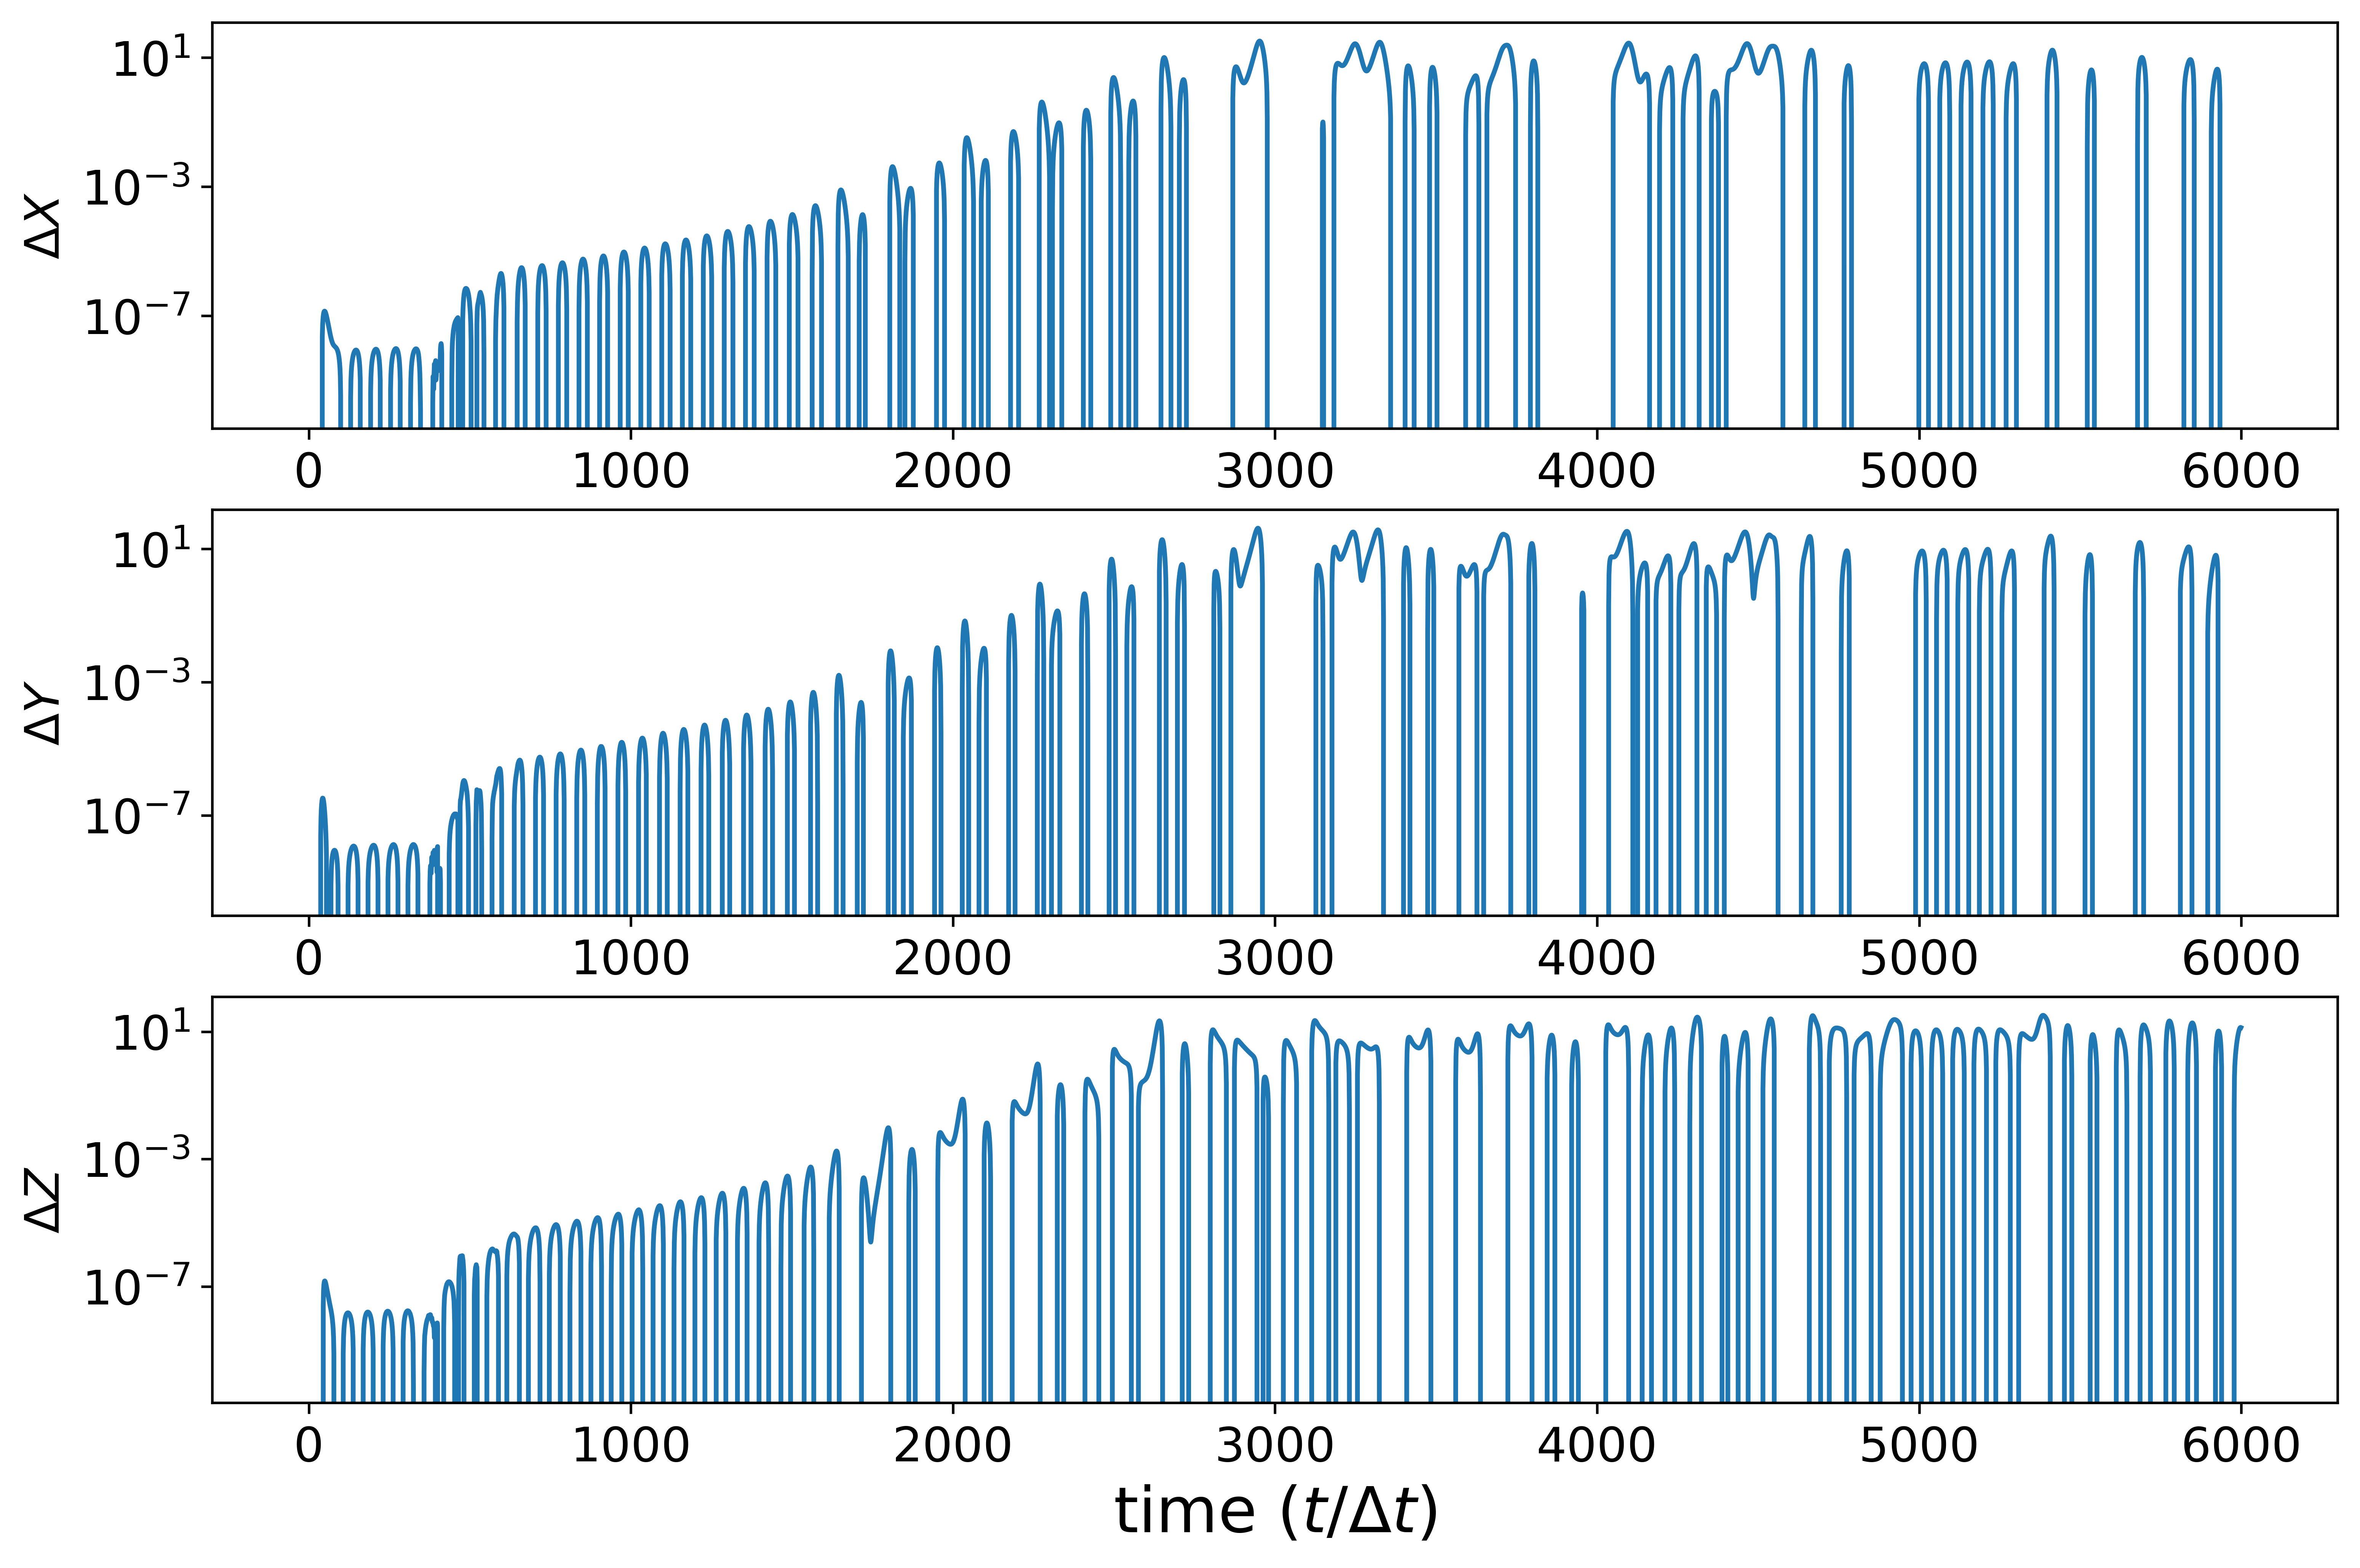
\includegraphics[scale = 0.6]{Figure_5.png}
    \caption{Plot of the difference between two different solution with slightly modified initial conditions.}
\end{figure}

Notice that the y axis is set to log scale in Figure 5. This means the linear growth between time = 0 and 3000 in Figure 5 corresponds to exponential growth in linear scale. Such exponentially growing divergence of nearby trajectories is a key feature of chaos.

\end{document}